\section{Study Area}
The study is conducted in the \textbf{Indus River Delta} (Fig.~\ref{fig:study_area}), located in the southern part of Sindh Province, Pakistan ($23.0^\circ\text{N}$ to $24.8^\circ\text{N}$, $67.0^\circ\text{E}$ to $69.0^\circ\text{E}$). The Indus Delta is a highly dynamic and ecologically vulnerable coastal wetland system, covering an area of approximately $30,000~\text{km}^2$. It is characterized by an arid to semi-arid climate, receiving less than $250~\text{mm}$ of annual rainfall, which occurs almost entirely during the summer monsoon (July--September).

\begin{figure}[t]
\centering
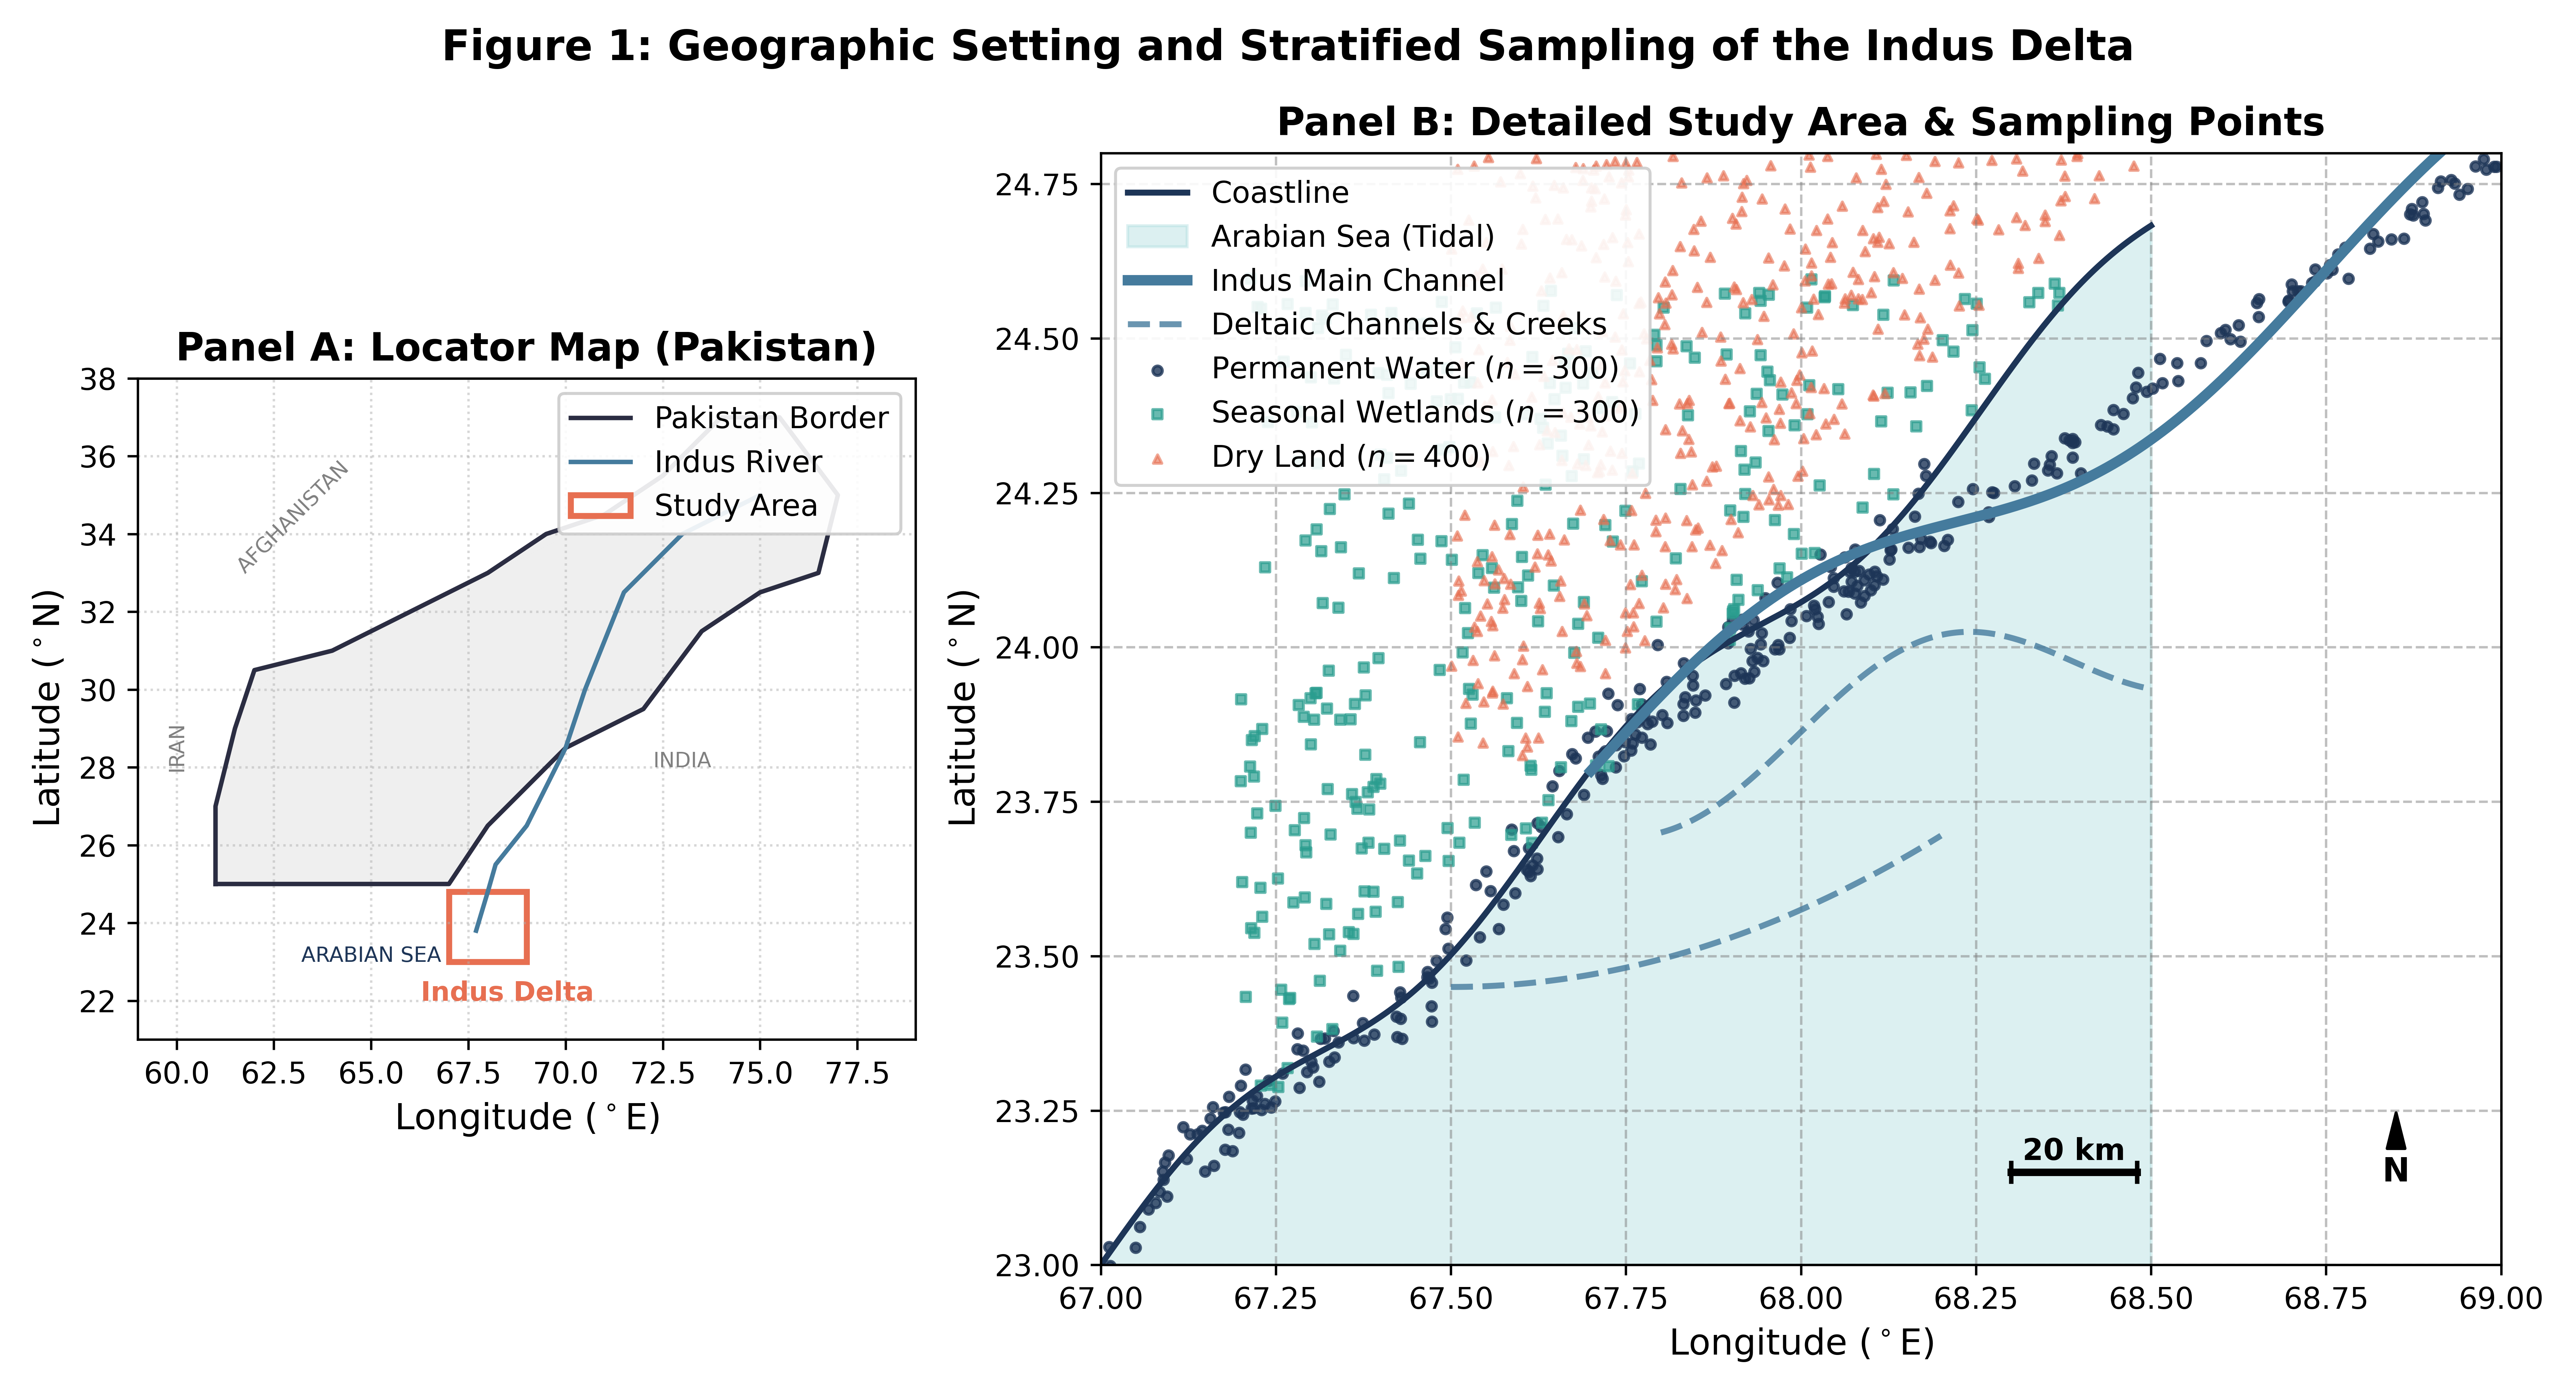
\includegraphics[width=0.95\linewidth]{figures/fig1_study_area.png}
\caption{Geographic setting and stratified point sampling design of the Indus River Delta. Panel A shows the locator map of Pakistan with the Indus River routing and the study area footprint. Panel B shows the detailed zoom-in of the delta, illustrating the coastline, main river channels, tidal creeks, and the distribution of the $1,000$ stratified random sampling points (permanent water, seasonal wetlands, and dry land) derived from historical JRC surface water occurrence.}
\label{fig:study_area}
\end{figure}

The deltaic hydrology is dominated by three main drivers:
\begin{enumerate}
    \item \textbf{Monsoonal Upstream Discharge:} The Indus River routes discharge from the Upper Indus Basin (meltwater from Hindu Kush-Karakoram-Himalayan glaciers and monsoon rainfall). This discharge is heavily regulated upstream by the Tarbela and Mangla reservoirs and a series of barrages. Historically, the river delivered a mean annual inflow of approximately $150~\text{billion cubic meters (BCM)}$ to the delta. However, extensive upstream diversions at the Kotri Barrage—the final downstream control structure—have reduced this to less than $10~\text{BCM}$ in normal years, though peak monsoonal floods (such as in 2022) can exceed $15,000~\text{m}^3~\text{s}^{-1}$.
    \item \textbf{Canal Irrigation Network:} A dense network of canals supplies freshwater to agricultural fields in the delta. The canal command area in the delta covers approximately $1~\text{million hectares}$, representing a highly managed sub-catchment where withdrawals redirect substantial freshwater volumes, creating localized surface water dynamics that are completely decoupled from local meteorological precipitation.
    \item \textbf{Coastal Tidal Inundation:} The delta's coastline is intersected by numerous creeks and mangrove wetlands subject to semi-diurnal tides with a mean tidal range of $2.0$ to $3.5~\text{m}$ at the coast. Seawater intrusion routes tidal head changes up to $80~\text{km}$ inland through topological pathways, affecting soil salinity and moisture persistence.
\end{enumerate}

During extreme meteorological anomalies (such as the historical 2022 Pakistan monsoon floods), river discharge exceeds barrage capacities, causing widespread inundation across the delta. In contrast, during normal dry seasons, active flow is confined to main channels and tidal creeks, while agricultural fields experience drydowns.
